\documentclass[12pt, letterpaper, preprint, comicneue]{aastex63}
%\usepackage[default]{comicneue} % comic sans font for editing
\usepackage[T1]{fontenc}
\input{vc}
\usepackage{color}
\usepackage{amsmath}
\usepackage{natbib}
\usepackage{ctable}
\usepackage{bm}
\usepackage[normalem]{ulem} % Added by MS for \sout -> not required for final version
\usepackage{xspace}
\usepackage{csvsimple} 

\usepackage{graphicx}
\usepackage{pgfkeys, pgfsys, pgfcalendar}


% typesetting shih
\linespread{1.08} % close to 10/13 spacing
\setlength{\parindent}{1.08\baselineskip} % Bringhurst
\setlength{\parskip}{0ex}
\let\oldbibliography\thebibliography % killin' me.
\renewcommand{\thebibliography}[1]{%
  \oldbibliography{#1}%
  \setlength{\itemsep}{0pt}%
  \setlength{\parsep}{0pt}%
  \setlength{\parskip}{0pt}%
  \setlength{\bibsep}{0ex}
  \raggedright
}
\setlength{\footnotesep}{0ex} % seriously?

% citation alias

% math shih
\newcommand{\setof}[1]{\left\{{#1}\right\}}
\newcommand{\given}{\,|\,}
\newcommand{\lss}{{\small{LSS}}\xspace}

\newcommand{\Om}{\Omega_{\rm m}} 
\newcommand{\Ob}{\Omega_{\rm b}} 
\newcommand{\OL}{\Omega_\Lambda}
\newcommand{\smnu}{M_\nu}
\newcommand{\sig}{\sigma_8} 
\newcommand{\mmin}{M_{\rm min}}
\newcommand{\BOk}{\widehat{B}_0} 
\newcommand{\hmpc}{\,h/\mathrm{Mpc}}
\newcommand{\bfi}[1]{\textbf{\textit{#1}}}
\newcommand{\parti}[1]{\frac{\partial #1}{\partial \theta_i}}
\newcommand{\partj}[1]{\frac{\partial #1}{\partial \theta_j}}
\newcommand{\mpc}{{\rm Mpc}}
\newcommand{\eg}{\emph{e.g.}}
\newcommand{\ie}{\emph{i.e.}}

% cmds for this paper 
\newcommand{\gr}{g{-}r}
\newcommand{\fnuv}{FUV{-}NUV}
\newcommand{\sfr}{{\rm SFR}}
\newcommand{\ssfr}{{\rm SSFR}}
\newcommand{\mtaum}{m_{\tau,M_*}}
\newcommand{\mtaus}{m_{\tau,{\rm SSFR}}}
\newcommand{\ctau}{c_\tau}
\newcommand{\mdeltam}{m_{\delta,M_*}}
\newcommand{\mdeltas}{m_{\delta,{\rm SFR}}}
\newcommand{\cdelta}{c_\delta}
\newcommand{\eda}{EDA}


\newcommand{\specialcell}[2][c]{%
  \begin{tabular}[#1]{@{}c@{}}#2\end{tabular}}
% text shih
\newcommand{\foreign}[1]{\textsl{#1}}
\newcommand{\etal}{\foreign{et~al.}}
\newcommand{\opcit}{\foreign{Op.~cit.}}
\newcommand{\documentname}{\textsl{Article}}
\newcommand{\equationname}{equation}
\newcommand{\bitem}{\begin{itemize}}
\newcommand{\eitem}{\end{itemize}}
\newcommand{\beq}{\begin{equation}}
\newcommand{\eeq}{\end{equation}}

%% collaborating
\newcommand{\todo}[1]{\marginpar{\color{red}TODO}{\color{red}#1}}
\definecolor{orange}{rgb}{1,0.5,0}
\newcommand{\ch}[1]{{\color{orange}{\bf CH:} #1}}

\begin{document} \sloppy\sloppypar\frenchspacing 

\title{PROVABGS Early Data Release: Probabilistic Stellar Mass Function} 
\date{\texttt{DRAFT~---~\githash~---~\gitdate~---~NOT READY FOR DISTRIBUTION}}

\newcounter{affilcounter}
\author{ChangHoon Hahn}
\altaffiliation{changhoon.hahn@princeton.edu}
\affil{Department of Astrophysical Sciences, Princeton University, Peyton Hall, Princeton NJ 08544, USA} 

\begin{abstract}
\end{abstract}

\keywords{
keyword1 -- keyword2 -- keyword3
}

% --- intro ---  
\input{intro}
% --- observations ---  
\section{The DESI Bright Galaxy Survey Early Data Release}  \label{sec:edr}


brief description of the DESI BGS early data release and fuji reduction 


We focus on BGS galaxies at $z < 0.3$. 

% --- methods ---  
\section{PROVABGS SED Modeling} \label{sec:provabgs}
% brief explanation of the PROVABGS SED modeling 
For each BGS EDR galaxy, we derive its $M_*$ and other properties,
$\overline{\rm SFR}$, $Z_{\rm MW}$, and $t_{\rm age, MW}$ from DESI
photometry and spectroscopy using the PROVABGS SED modeling
framework~\citep{hahn2022}.  
PROVABGS models galaxy SEDs using stellar population synthesis with
non-parametric star-formation history (SFH) with a starburst, a non-parametric
metallicity history (ZH) that varies with time, and a flexible dust
attenuation prescription.
The non-parameteric SFH and ZH prescriptions are derived from SFHs and ZHs of
simulated galaxies in the Illustris hydrodynamic
simulation~\citep{vogelsberger2014, genel2014, nelson2015} and provide compact 
and flexibly representations of SFHs and ZHs.
For the stellar population synthesis, PROVABGS uses the Flexible Stellar
Population Synthesis~\citep[FSPS;][]{conroy2009, conroy2010b} model with MIST
isochrones~\citep{paxton2011, paxton2013, paxton2015, choi2016, dotter2016},
\cite{chabrier2003} initial mass function (IMF), and a combination of
MILES~\citep{sanchez-blazquez2006} and BaSeL~\citep{lejeune1997, lejeune1998,
westera2002} spectral libraries.

Furthermore, PROVABGS provides a Bayesian inference framework for inferring
full posterior probability distributions of the SED model parameter:
$p(\theta\given {\bf X}^{\rm photo}, {\bf X}^{\rm spec})$, where ${\bf X}^{\rm
photo}$ represents the photometry and ${\bf X}^{\rm spec}$ represents the
spectroscopy. 
In total, $\theta$ has 13 parameters: $M_*$, 6 parameters specifying the SFH
($\beta_1, \beta_2, \beta_3, \beta_4, f_{\rm burst}, t_{\rm burst}$), 2
parameters specifying ZH ($\gamma_1, \gamma_2$), 3 parameters specifying
dust attenuation ($\tau_{\rm BC}, \tau_{\rm ISM}, n_{\rm dust}$), and a
nuisance parameter for the fiber aperture effect. 
Posteriors have distinct advantages over point estimates because they
accurately estimate uncertainties and degeneracies among galaxy properties.
Furthermore, as we later demonstrate, they are essential for principled
population inference: \eg~SMF.  

In practice, accurately estimating a 13 dimensional posterior requires a large
number ($\gtrsim$100,000) SED model evaluations, which would require
prohibitive computational resources. 
To address this challenge, PROVABGS samples the posterior using the
\cite{karamanis2020} ensemble slice Markov Chain Monte Carlo (MCMC) sampling
with the {\sc zeus} Python package\footnote{https://zeus-mcmc.readthedocs.io/}.
PROVABGS further accelerates the inference by using neural emulators for the
SED models. 
The emulators are accurate to subpercent level and $>100\times$ faster than the
original SED model based on FSPS~\citep{kwon2022}. 
With {\sc zeus} and neural emulation, deriving a posterior takes $\sim$5 min
per galaxy with PROVABGS.
Moreover, \cite{hahn2022} demonstrated PROVABGS can accurately infer $M_*$
overall the full expected $M_*$ range of BGS, using forward modeled synthetic
DESI observations. 

\begin{figure}
\begin{center}
    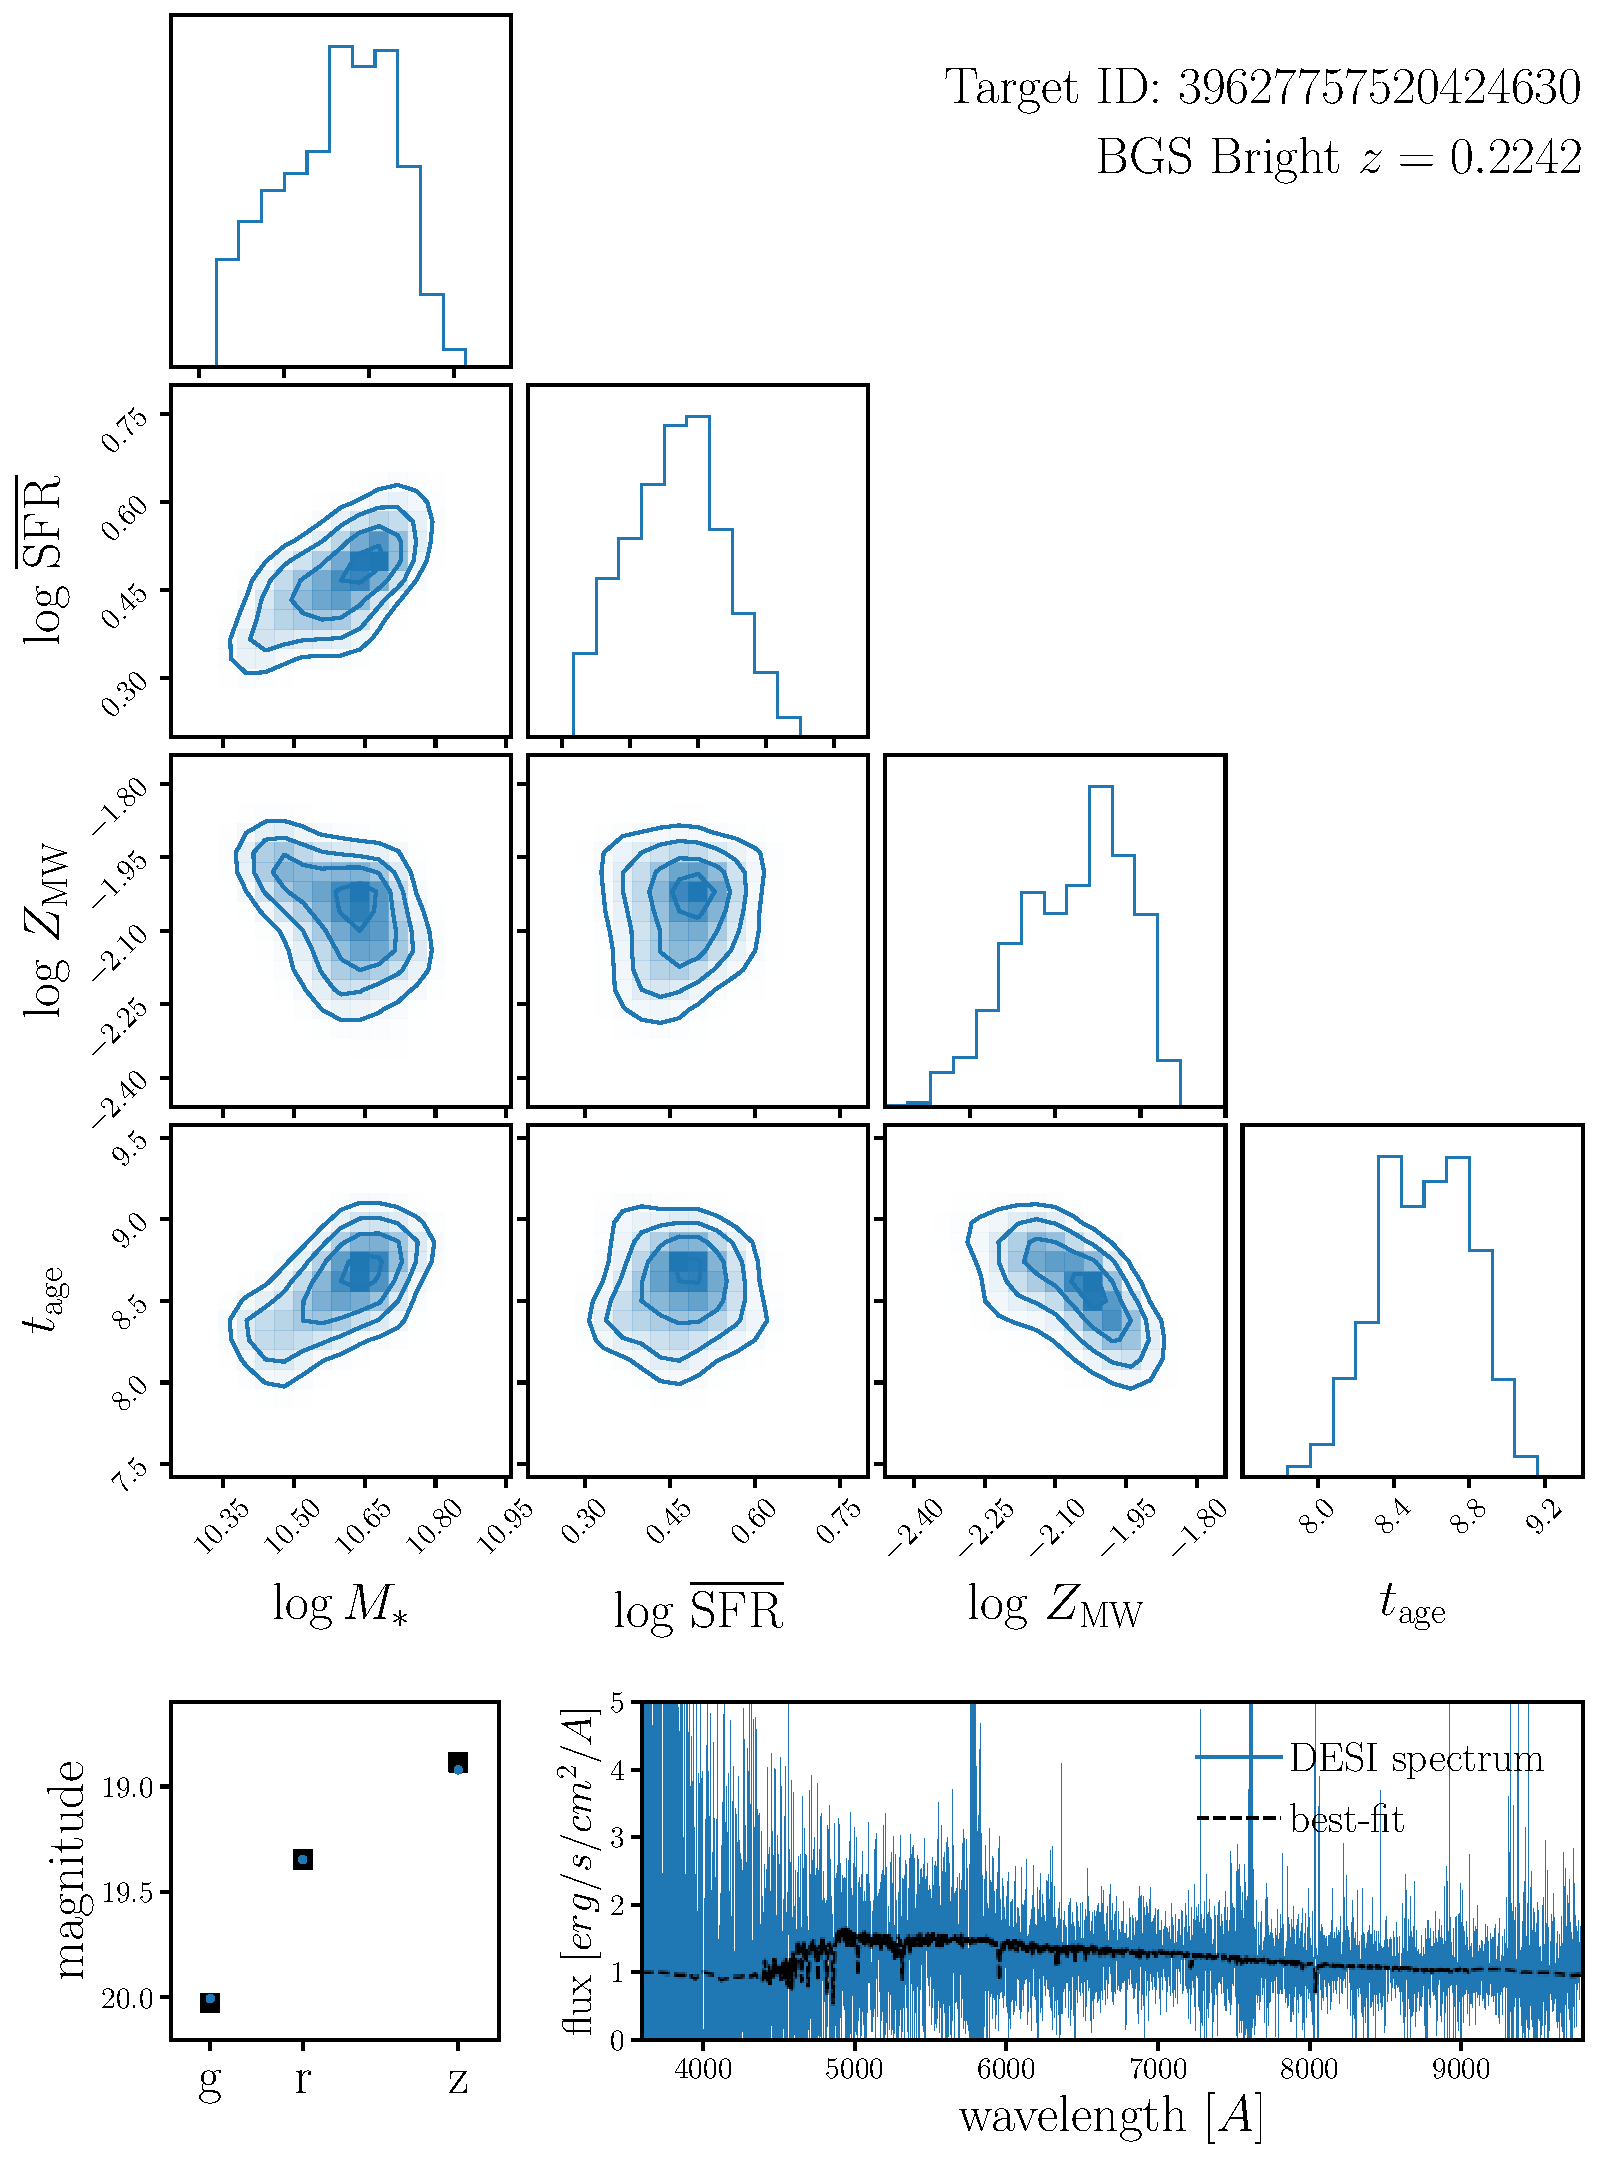
\includegraphics[width=0.6\textwidth]{figs/provabgs_posterior.pdf}
    \caption{
    }\label{fig:posterior}
\end{center}
\end{figure}


\begin{figure}
\begin{center}
    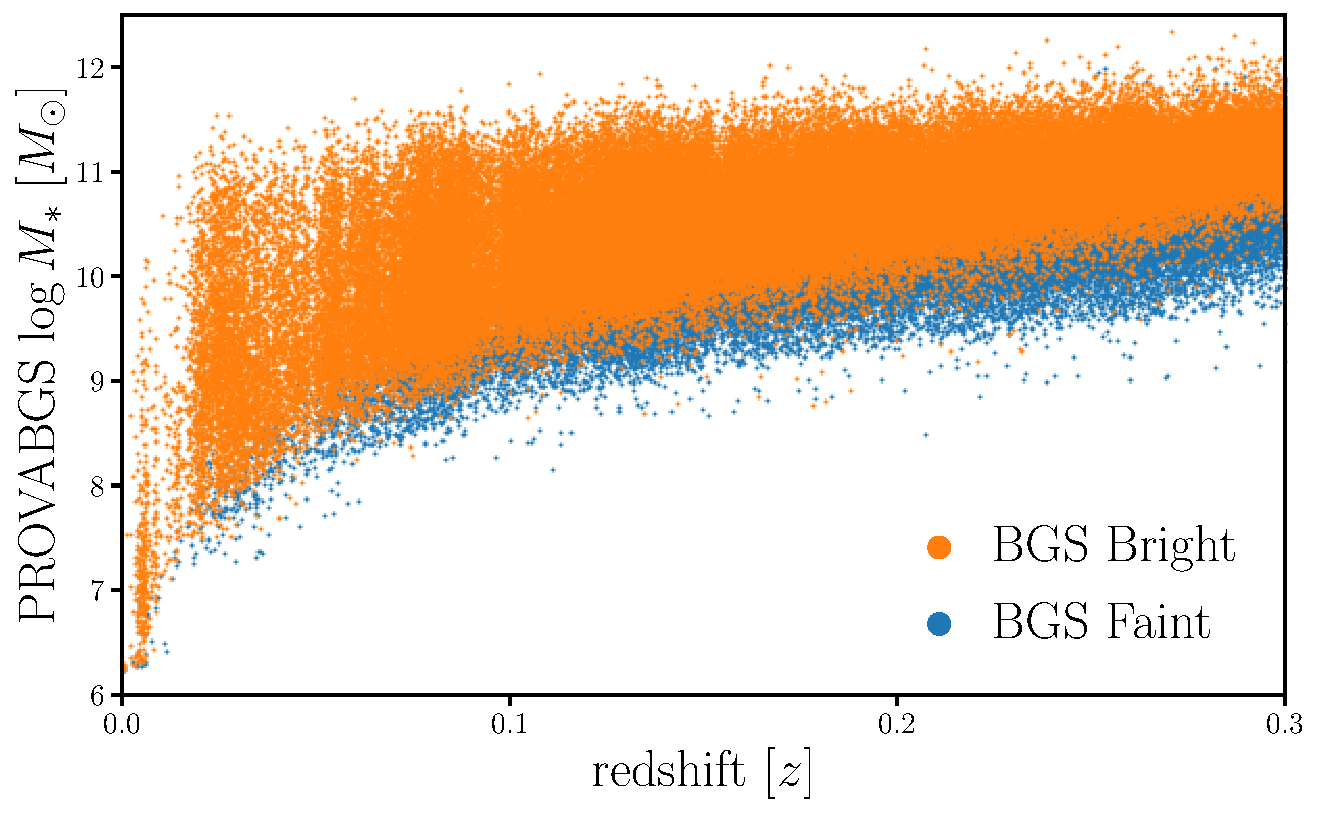
\includegraphics[width=0.6\textwidth]{figs/mstar_z.pdf}
    \caption{
    }\label{fig:mstar_z}
\end{center}
\end{figure}


In Figure~\ref{fig:posterior}, 

Figure~\ref{fig:mstar_z},

% --- results ---  
\section{Results} \label{sec:results}
We are interested in estimating the SMF of BGS galaxies from their individual
marginalized posteriors, $p(M_* \given {\bfi X_i})$, derived using
PROVABGS~(Section~\ref{sec:provabgs}). 

we're going to do population inference in a hierarchical bayesian framework and
use a normalizing flow.
%We can infer the population hyperparameters, μ∆θ and σ∆θ , using a hierarchical Bayesian framework (e.g. Hogg et al. 2010; Foreman-Mackey et al. 2014; Baronchelli et al. 2020).

why? because it produces unbiased inference. 

why do we use normalizing flows? 

We follow the same approach as \cite{hahn2022} to estimate:
\begin{align}\label{eq:popinf}
p(\phi \given \{{\bfi X_i}\}) 
    =&~\frac{p(\phi)~p( \{{\bfi X_i}\} \given \phi)}{p(\{{\bfi X_i}\})}\\
    =&~\frac{p(\phi)}{p(\{{\bfi X_i}\})}\int p(\{{\bfi X_i}\} \given \{\theta_i\})~p(\{\theta_i\} \given \phi)~{\rm d}\{\theta_i\}.\\
    =&~\frac{p(\phi)}{p(\{{\bfi X_i}\})}\prod\limits_{i=1}^N\int p({\bfi X_i} \given \theta_i)~p(\theta_i \given \phi)~{\rm d}\theta_i\\
    =&~\frac{p(\phi)}{p(\{{\bfi X_i}\})}\prod\limits_{i=1}^N\int \frac{p(\theta_i \given {\bfi X_i})~p({\bfi X_i})}{p(\theta_i)}~p(\theta_i \given \phi)~{\rm d}\theta_i\\
    =&~p(\phi)\prod\limits_{i=1}^N\int \frac{p(\theta_i \given {\bfi X_i})~p(\theta_i \given \phi)}{p(\theta_i)}~{\rm d}\theta_i. 
\intertext{
    We estimate the integral using $S_i$ Monte Carlo samples from the
    individual posteriors $p(\theta_i \given {\bfi X_i})$: 
}
    \approx&~p(\phi)\prod\limits_{i=1}^N\frac{1}{S_i}\sum\limits_{j=1}^{S_i}
    \frac{p(\theta_{i,j} \given \phi)}{p(\theta_{i,j})}.
\end{align} 

BGS provides two samples: BGS Bright and Faint. 
Galaxies in BGS Bright are selected based on a $r < 19.5$ flux limit, while
the ones in BGS Faint are selected based on a fiber-magnitude and color limit
and $r < 20.0175$ flux limit. 
Since neither of these samples are volume-limited and complete as a function
of $M_*$, we must include the selection effect when estimating the SMF. 
We do this by including weights derived from $z^{\rm max}$, the maximum
redshift that galaxy $i$ could be placed and still be included in the BGS
samples. 
We derive $z^{\rm max}_i$ for every galaxy using by redshifting the SED
predicted by the best-fit parameters. 
We then derive $V^{\rm max}_i$, the comoving volume out to $z^{\rm max}_i$, and
weights $w_i = w_{i, {\rm comp}}/V^{\rm max}_i$. 
We modify Eq.~\ref{eq:popinf} to include $w_i$: 
\begin{align}
p(\phi \given \{{\bfi X_i}\}) 
    \approx&~\frac{p(\phi)}{\prod\limits_{i=1}^N p({\bfi X_i})^{w_i}} 
    \prod\limits_{i=1}^N \left(\int p({\bfi X_i} \given \theta_i)~p(\theta_i \given \phi)~{\rm d}\theta_i \right)^{w_i} \\ 
    \approx&~\frac{p(\phi)}{\prod\limits_{i=1}^N p({\bfi X_i})^{w_i}} 
    \prod\limits_{i=1}^N \left( \sum\limits_{j=1}^{S_i}
    \frac{p(\theta_{i,j} \given \phi)}{p(\theta_{i,j})} \right)^{w_i} \\
    \approx&~\frac{p(\phi)}{\prod\limits_{i=1}^N p({\bfi X_i})^{w_i}} 
    \prod\limits_{i=1}^N \left( \sum\limits_{j=1}^{S_i}
    \frac{q_\phi(\theta_{i,j})}{p(\theta_{i,j})} \right)^{w_i}.
\end{align} 

In practice, we do not derive the full posterior 
$p(\phi \given \{{\bfi X_i}\})$. 
Instead we derive the maximum a posteriori (MAP) hyperparameter 
$\phi_{\rm MAP}$ that maximizes $p(\phi \given \{{\bfi X_i}\})$ or 
$\log p(\phi \given \{{\bfi X_i}\})$.
We expand, 
\begin{align}
\log p(\phi \given \{{\bfi X_i}\}) 
    \approx&~\log p(\phi) + % \sum\limits_{i=1}^N w_i \log w_i + 
    \sum\limits_{i=1}^N w_i \log \left(\sum\limits_{j=1}^{S_i} \frac{q_\phi(\theta_{i,j})}{p(\theta_{i,j})} \right).
\end{align} 
Since the first two terms are constant, we derive $\phi_{\rm MAP}$ by
maximizing 
\begin{equation}
    \max_\phi~~\sum\limits_{i=1}^N w_i \log \left(\sum\limits_{j=1}^{S_i} \frac{q_\phi(\theta_{i,j})}{p(\theta_{i,j})} \right).
\end{equation}
We use {\sc Adam} optimizer and determine the architecture of the normalizing
flow through experimentation.  


%\approx&~\log p(\phi) - 
%\log \prod\limits_{i=1}^N p({\bfi X_i})^{w_i} + 
%\log \prod\limits_{i=1}^N \left(\int p({\bfi X_i} \given \theta_i)~p(\theta_i \given \phi)~{\rm d}\theta_i \right)^{w_i} \\
%\approx&~\log p(\phi) - 
%\sum\limits_{i=1}^N w_i \log p({\bfi X_i}) + 
%\sum\limits_{i=1}^N w_i \log \left(\int p({\bfi X_i} \given \theta_i)~p(\theta_i \given \phi)~{\rm d}\theta_i \right) \\
%\approx&~\log p(\phi) + 
%\sum\limits_{i=1}^N w_i \log \left(\frac{1}{w_i} \sum\limits_{j=1}^{S_i} w_{i,j} \frac{p(\theta_{i,j} \given \phi)}{p(\theta_{i,j}} \right) \\


%\subsection{Targeting Completeness} \label{sec:ts}
% https://desi.lbl.gov/trac/wiki/ClusteringWG/LSScat/SV3/version2.1/fulldat
% https://desi.lbl.gov/trac/wiki/ClusteringWG/LSScat/SV3/version2.1/fullran
\subsection{Spectroscopic Completeness} \label{sec:spec_comp}
% https://desi.lbl.gov/trac/wiki/ClusteringWG/LSScat/DA02main/current_version#clusteringfiles
fiber assignment completeness: weights available from the alternate MTLs


redshift failure weights based on TSNR2 and fiber flux 

\subsection{The Probabilistic Stellar Mass Function} \label{sec:psmf}


% --- summary ---  
\input{summary}

\section*{Acknowledgements}
It's a pleasure to thank

\appendix
\section{Stellar Mass Completeness} \label{sec:mscomp}

First, we take galaxies with $i \Delta z < z < (i+1) \Delta z$. 

For each galaxy take their best-fit SED from {\sc PROVABGS} and artificially redshift it to 
$z' = z + \Delta z$.

afterward, calculate the $r$ band magnitude using the best-fit SED and
determine whether the galaxy at $z'$ would be within the target selection. 


We then compare the $M_*$ distributions and determine the $M_*$ below which  a
significant number of galaxies are excluded from the sample.  


\bibliographystyle{mnras}
\bibliography{psmf} 
\end{document}
